\begin{frame}
\titlepage{}
\end{frame}

\section{Общая характеристика работы}

\begin{frame}
\frametitle{Требования и ограничения}

Требования и ограничения, предъявляемые к решению:
\begin{wrapfigure}{r}{0.5\textwidth}
	\centering
    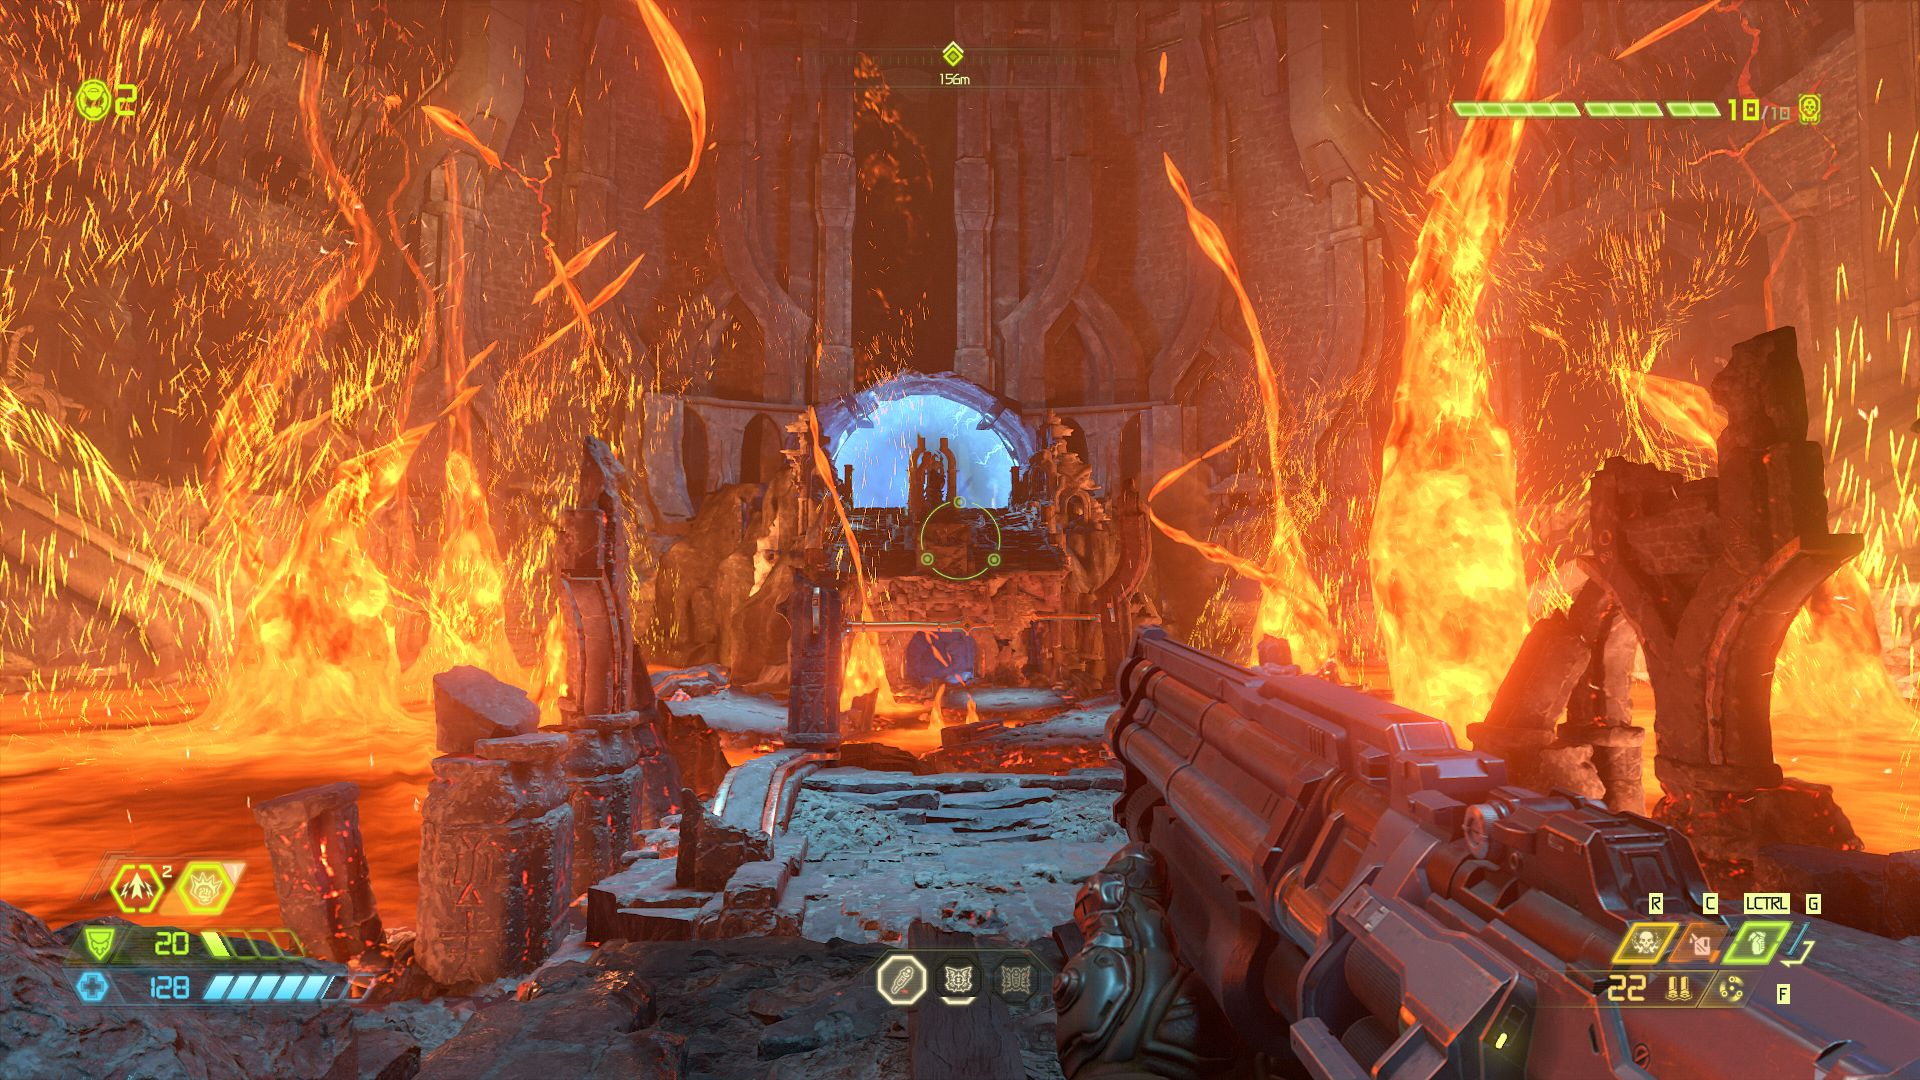
\includegraphics[width=0.5\textwidth]{DoomEternal}
    \caption{Кадр из игры Doom Eternal}%
    \label{fig:doomEternal}
\end{wrapfigure}
\begin{itemize}
    \item средняя частота кадров сцены --- 60 кадров /сек.;
    \item максимальная визуальная привлекательность;
    \item адаптивность под задачи художников.
\end{itemize}
\end{frame}

\section{Анализ литературных источников}
\begin{frame}
\frametitle{Классификация методов симуляции огня}

\begin{table}[htb]
    \caption{Сравнение производительности различных методов симуляции огня}
    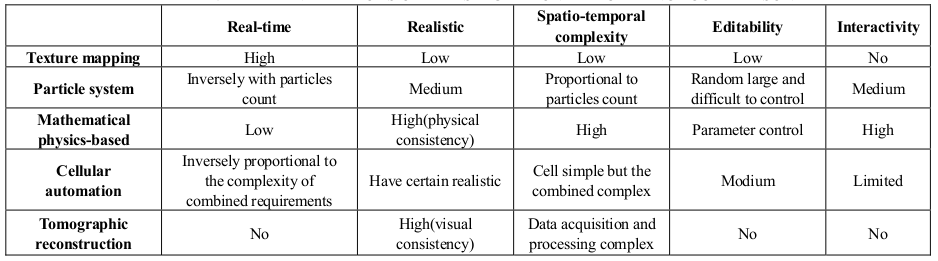
\includegraphics[width=\textwidth]{simulation_methods}%
    \label{table:algoAnalsysis}
\end{table}
\end{frame}

\section{Теория динамической симуляции огня}
\begin{frame}[t]
\frametitle{Структура симуляции}
\begin{wrapfigure}{r}{0.5\textwidth}
	\centering
    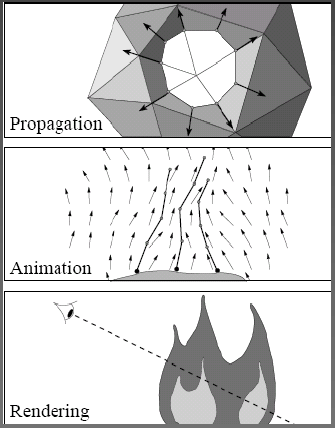
\includegraphics[width=0.4\textwidth]{simStages}
    \caption{Структура симуляции}%
    \label{fig:simStages}
\end{wrapfigure}
Компоненты симуляции:
\begin{itemize}
	\item моделирование;
	\item анимация;
	\item визуализация.
\end{itemize}
Альтернативная схема была предложена Филиппом Боденом (рис.~\ref{fig:simStages}).
\end{frame}

\subsection{Компоненты решения}
\begin{frame}
\frametitle{Структура симуляции}
\begin{figure}[htb]
	\centering
	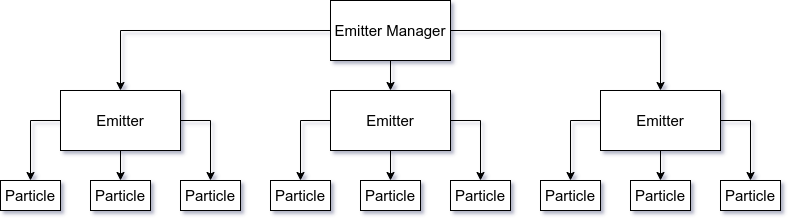
\includegraphics[width=\textwidth]{Structure}
    \caption{Иерархия объектов, использованная в разработанном симуляторе}%
    \label{fig:simStructure}
\end{figure}
\end{frame}

\begin{frame}
\frametitle{Использованные инструменты}
\begin{itemize}
    \item Язык программирования: C++;
    \item Графический интерфейс: OpenGL v4.5;
    \item Язык написания шейдеров: GLSL.
\end{itemize}
\begin{figure}
	\centering
    
\includegraphics[width=0.3\textwidth]{opengl}
    \caption{Логотип OpenGL}%
    \label{fig:opengl}
\end{figure}
\end{frame}

\begin{frame}
\frametitle{Схема обновления частиц}
\begin{figure}
	\centering
	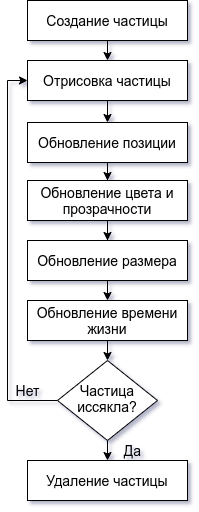
\includegraphics[height=7.1cm]{algorithm2}
    \caption{Схема обновления частиц в кадре}%
    \label{fig:algorithm}
\end{figure}
\end{frame}

\begin{frame}
\frametitle{Промежуточные результаты}
\begin{wrapfigure}{r}{0.4\textwidth}
	\centering
    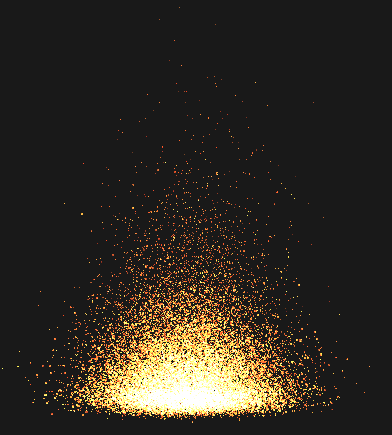
\includegraphics[width=0.3\textwidth]{proto4}
    \caption{''Наивная'' анимация}%
    \label{fig:proto4}
\end{wrapfigure}

Уравнения движения:
\begin{align}
  \label{eq:position}
  \vec{p}(t + \Delta{t}) &= \vec{p}(t) + \vec{v}(t) \cdot \Delta{t} \\
  \label{eq:velocity}
  \vec{v}(t + \Delta{t}) &= \vec{v}(t) + \vec{a} \\
  \label{eq:accelearation}
  \vec{a} &= 0,02 \cdot \vec{v}_{0}
\end{align}
\end{frame}

\begin{frame}
\frametitle{Анимация частиц}
\begin{figure}
	\centering
    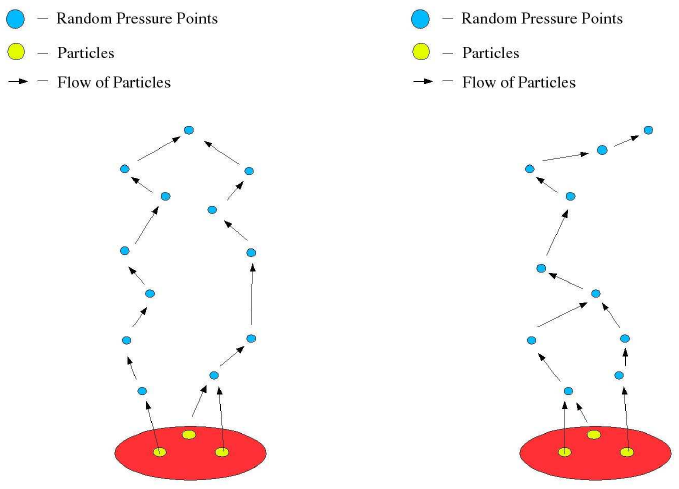
\includegraphics[width=0.75\textwidth]{animationAlgo}
    \caption{Алгоритм анимации частиц}%
    \label{fig:animationAlgo}
\end{figure}
\end{frame}

\begin{frame}[t]
\frametitle{Реализация анимации}
\begin{wrapfigure}{r}{0.3\textwidth}
	\centering
    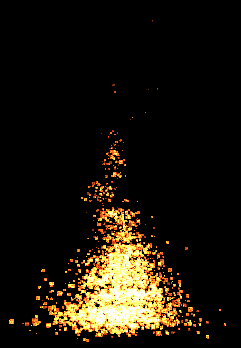
\includegraphics[width=0.3\textwidth]{protoFinal}
    \caption{Реализация анимации частиц}%
    \label{fig:protoFinal}
\end{wrapfigure}
Сложность алгоритма:
\begin{equation}
    O(n \log n) + O(m) \cdot O(\log_{2} n)
\end{equation}
\begin{explanationx}
    \item [где] $n$ --- количество точек низкого давления;
    \item $m$ --- количество частиц.
\end{explanationx}
\end{frame}

\begin{frame}[t]
\frametitle{Текстурные сплэты}
\begin{wrapfigure}{r}{0.3\textwidth}
	\centering
    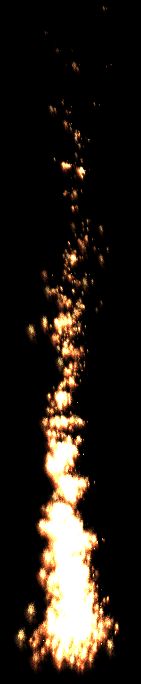
\includegraphics[height=5.5cm]{simSplats}
    \caption{Использование текстурных сплэтов для рендеринга частиц}%
    \label{fig:protoSplats}
\end{wrapfigure}
Преимущества метода:
\begin{itemize}
    \item оптимизация количества частиц;
    \item увеличение детализации за счет текстур;
    \item более плавная форма пламени.
\end{itemize}

Недостатки метода:
\begin{itemize}
    \item необходимо ориентировать полигоны на зрителя;
    \item нереалистичные результаты при наблюдении сверху.
\end{itemize}
\end{frame}

\subsection{Экспериментальные результаты}
\begin{frame}[allowframebreaks]
\frametitle{Сравнение с аналогами}
''Fire Simulation
in 3D Computer Animation with Turbulence Dynamics including Fire Separation and
Profile Modeling'' (2018 год).
\begin{figure}[htb]
	\centering
    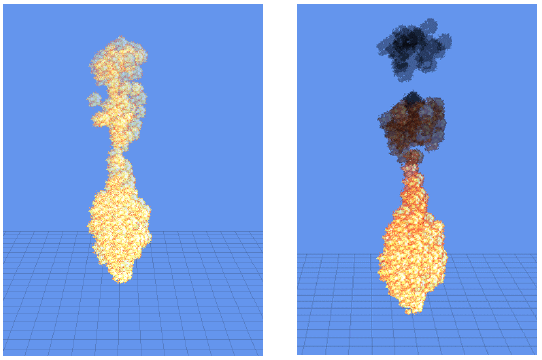
\includegraphics[width=0.7\textwidth]{turbulence}
    \caption{Результаты работы системы}%
    \label{fig:turbulence}
\end{figure}

Тестовая среда:
\begin{itemize}
    \item \textbf{ЦП}: Intel Core i3 350m 2.26ГГц;
    \item \textbf{ГП}: ATI Radeon 5145;
    \item \textbf{ОЗУ}: 4 ГБ.
\end{itemize}

Эксперимент:
\begin{itemize}
    \item 1 сплайн;
    \item 15 сегментов в сплайне;
    \item по 100 частиц в каждом сегменте;
    \item 30+ кадров в секунду.
\end{itemize}
\end{frame}

\begin{frame}
\frametitle{Производительность системы}
Тестовая среда:
\begin{itemize}
    \item \textbf{ЦП}: Intel Core i5--5200U 2.7ГГц;
    \item \textbf{ГП}: Intel HD Graphics 5500;
    \item \textbf{ОЗУ}: 8 ГБ;
    \item \textbf{ОС}:Debian 10 Buster.
\end{itemize}

\begin{table}[htb]
\caption{Зависимость частоты кадров от количества частиц в системе}%
\label{table:amountBench}
\centering
\small
\begin{tabular}{| l | l |}
    \hline
    Количество частиц & Средняя частота кадров \\
    \hline
    5000 &  60,00 \\
    \hline
    10000 & 58,46 \\
    \hline
    15000 & 50,62 \\
    \hline
    25000 & 31,94 \\
    \hline
    50000 & 15,85 \\
    \hline
\end{tabular}
\end{table}
\end{frame}

\section{Заключение}
\begin{frame}
\frametitle{Заключение}
\begin{itemize}
    \item разработана система симуляции огня для приложений реального времени;
    \item использованная комбинация системы частиц и метода текстурного
        сплэттинга позволила улучшить качество визуализации и оптимизировать
        количество частиц;
    \item реализованный метод анимации позволил добиться эффектной анимации
        частиц при низких вычислительных затратах;
    \item разработанная система может быть использована в видеоиграх.
\end{itemize}
\end{frame}

\section{Библиографический список}
\begin{frame}[t,allowframebreaks]
\frametitle{Список публикаций соискателя}
\nocite{*}
\sloppy\printbibliography[
    category=AuthorSources,
    heading=none,
    resetnumbers,
]
\end{frame}
